\documentclass{beamer}
\usepackage[brazilian]{babel}
\usepackage[utf8]{inputenc}
\usepackage[T1]{fontenc}
\usepackage{array}
\usepackage{listings}

\usetheme{Laughlin}

\begin{document}
\title{Algoritmo não Supervisionado para Segmentação e Remoção de
Ruído de Páginas \textit{web} Utilizando \textit{tag paths}}
%\author[Roberto Panerai Velloso]{Orientando: Roberto Panerai Velloso \\
%Orientadora: Carina F. Dorneles \\ \{rvelloso, dorneles\}@gmail.com }
\author[Roberto Panerai Velloso]{Roberto Panerai Velloso, Carina F. Dorneles \\ 
\{rvelloso, dorneles\}@gmail.com}
%\date{\today}
\date{}
%\institute{Universidade Federal de Santa Catarina}
\institute{
%UFSC - Universidade Federal de Santa Catarina \\ PPGCC - Programa de
% Pós-Graduação em Ciência da Computação
\begin{figure}[H]
  \label{fig:logo1}
    
\includegraphics[scale=0.50]{img/brasao_ufsc_80.png}
    
\includegraphics[scale=0.30]{img/brasao_418.jpg}
\end{figure}
%\begin{figure}[H]
%  \label{fig:logo2}
%    
\includegraphics[scale=0.30]{brasao_ufsc_80.png}
%\end{figure}
}

\frame{
\titlepage
} 

\frame{\frametitle{Sumário}\tableofcontents}

\section{Introdução} 
%\frame{\tableofcontents[currentsection]}
\frame{\frametitle{Introdução}
\begin{itemize} 
	\item Data mining na web (relevância);
	\begin{itemize}
	\item Usage mining (sistemas de recomendação)
	\item IR (indexing, clustering \& Análise de hyperlinks)
	\item \textit{Deep web/surfacing}
	\item Extração estruturada
	\end{itemize}
	\item Contexto do trabalho
	\begin{itemize}
	\item Extração estruturada
	\item Remoção de ruído (importância)
	\end{itemize}
\end{itemize}
}

\frame{\frametitle{Problema - remoção de ruído}
\begin{itemize} 
	\item Ruído: anúncios, menus, $template$, etc;
	\item Identificar a região principal de uma página $web$, com o objetivo de
	eliminar o restante da página (ruído) antes da fase de extração dos dados;
	\item Etapa de limpeza é fundamental para obtenção de resultados satisfatórios
	na fase de extração de dados;
	\item Ruído representa parcela considerável dos dados na \textit{web};
	\item Poucos trabalhos na área (LIU; CHANG, 2004).
\end{itemize}
}

\frame{\frametitle{Problema - remoção de ruído}
\begin{figure}[H]
  %\caption{Exemplo de uma página web com a região principal delimitada
  %HTML.}
  \label{fig:ex2}
  \centering
    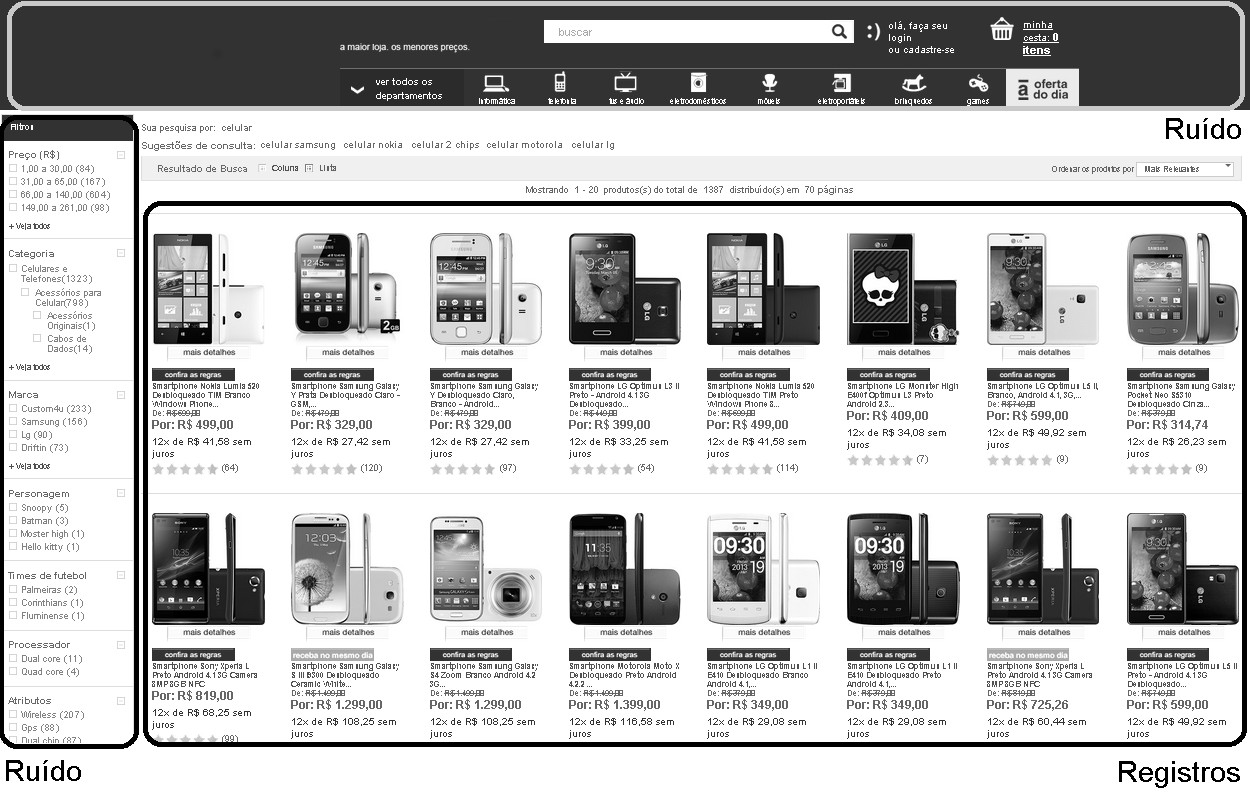
\includegraphics[scale=0.20]{img/exemploruido.jpg}
\end{figure}
}

\frame{\frametitle{Problema - remoção de ruído}
\begin{figure}[H]
  %\caption{Exemplo de uma página web com a região principal delimitada
  %HTML.}
  \label{fig:ex2}
  \centering
    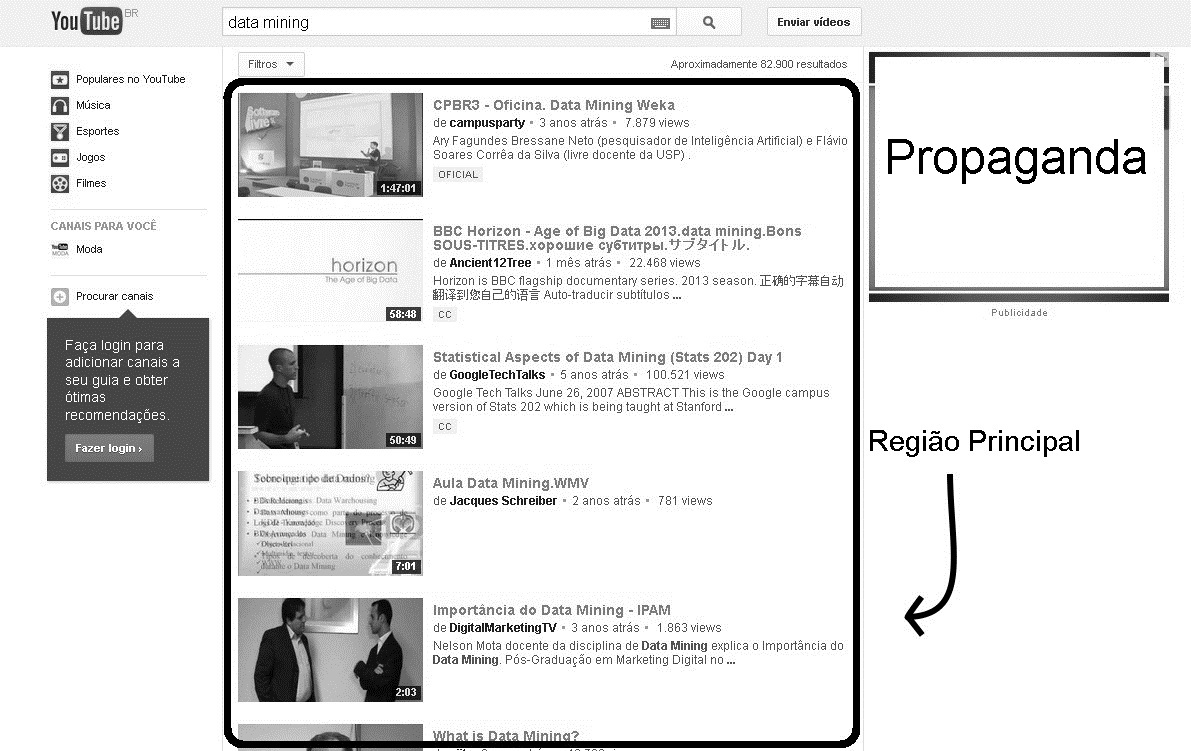
\includegraphics[scale=0.29]{img/example2-gs-pt.jpg}
\end{figure}
}

\section{Objetivo} 
%\frame{\tableofcontents[currentsection]}
\frame{\frametitle{Objetivo} 
Contribuir para a área de extração estruturada de dados da $web$ com uma nova
técnica de remoção de ruído que possibilite incrementar a precisão dos métodos
de extração e que tenha as seguintes características:
\begin{itemize}
  \item Independente de domínio;
  \item Independente de características da linguagem HTML; 
  \item Não dependa de bases de dados e/ou definições $a$ $priori$.
  \item Totalmente automática;
  \item Necessite de apenas uma página (ao invés de um conjunto de páginas);
  \item Não dependa de treinamento;
\end{itemize}
}
\section{Trabalhos correlatos} 
%\frame{\tableofcontents[currentsection]}
\frame{\frametitle{Trabalhos correlatos} 
\begin{tiny}
\begin{table}[h]
\centering
\caption{Comparativo entre técnicas de segmentação de página}
\label{table:comp}
\begin{tabular}{p{0.01cm}|p{2.5cm} p{0.5cm} p{0.5cm} p{0.5cm} p{1cm} p{0.5cm}
p{0.8cm}} \hline\hline
\# 
&Técnica   
&Entrada
&Única página   
&Treina-mento     
&Informação a priori 
&Indep. HTML 
&Abordagem \\
\hline
1 & Kohlschutter e Nejdl (2008) & Texto & - & - & - & - & Densid. Textual\\
2 & Kohlschutter, Fankhauser e Nejdl (2010) & Texto & - & - & - & - & \textit{Decision tree}\\
3 & Weninger, Hsu e Han (2010) & Texto & - & - & - & - & \textit{Clustering} e limiar\\
4 & Yi, Liu e Li (2003) & DOM & Não & Sim & Não & Sim & Heurística\\
5 & Chakrabarti, Kumar e Punera (2008) & DOM & Não & Sim & Não & Sim & Grafos \\
6 & Cho, Lin e Kao (2009) & DOM & Sim & Não & Sim & Não & Entropia\\
7 & Fernandes et al. (2011) & DOM & Não & Sim & Não & Sim & Heurística\\
8 & Zheng, Gu e Li (2012) & DOM & Sim & Não & Sim & Sim & Entropia Semântica\\
9 & Lutz e Heuser (2013) & DOM & Não & Sim & Não & Sim & \textit{Decision tree}\\
10 & Cai et al. (2003) & Visual & Sim & Não & Sim & Não & Conjunto de regras\\
11 & Simon e Lausen (2005) & Visual & Sim & Não & Não & Sim & Distância \\
12 & Fernandes et al. (2007) & Visual & Não & Sim & Não & Não & Estatística\\
13 & Liu, Meng e Meng (2010) & Visual & Sim & Não & Sim & Não & \textit{Clustering}\\
\hline
14 & Velloso e Dorneles (2013) & TPS & Sim & Não & Não & Sim & Seg. TPS\\
\end{tabular}
\end{table}
\end{tiny}
}
\subsection{$Tag$ $paths$}

\frame{\frametitle{$Tag$ $paths$}
\begin{small}
Miao et al. (2009) e Xie et al. (2012)
\begin{figure}[H]
  \caption{Construção da seqüência de $tag$ $paths$ (TPS) a partir do HTML.}
  \label{fig:ex1}
  \centering
    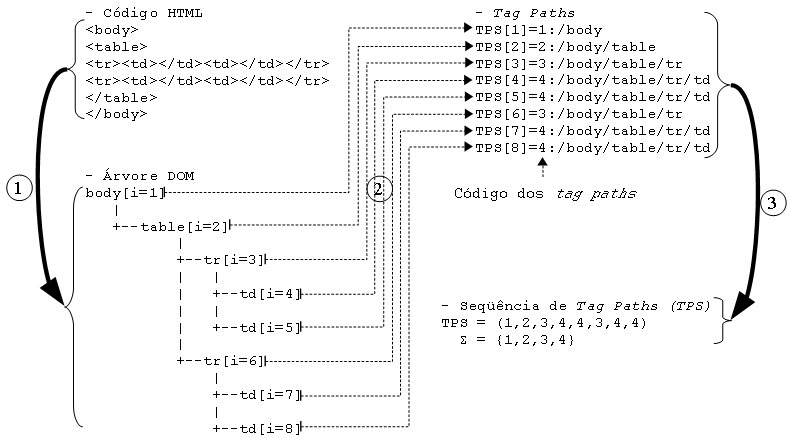
\includegraphics[scale=0.45]{img/example1-pt.jpg}
\end{figure}
\end{small}
}
\section{Hipótese} 
%\frame{\tableofcontents[currentsection]}
\frame{\frametitle{Hipótese}
\begin{enumerate}
	\item Diferentes regiões de uma página $web$ são descritas utilizando diferentes
	$tag$ $paths$;
	\item Em páginas com conteúdo semi-estruturado (i.e. registros, como definido
	em Liu, Grossman e Zhai (2003)), a região principal é estruturalmente mais
	densa/maior que as demais regiões da página (menus, anúncios, texto, etc.).
\end{enumerate} 
}
\subsection{Algoritmo}

\frame{\frametitle{Algoritmo}
\begin{figure}[H]
  \caption{Ilustração da execução do algoritmo.}
  \label{fig:alg}
  \centering
    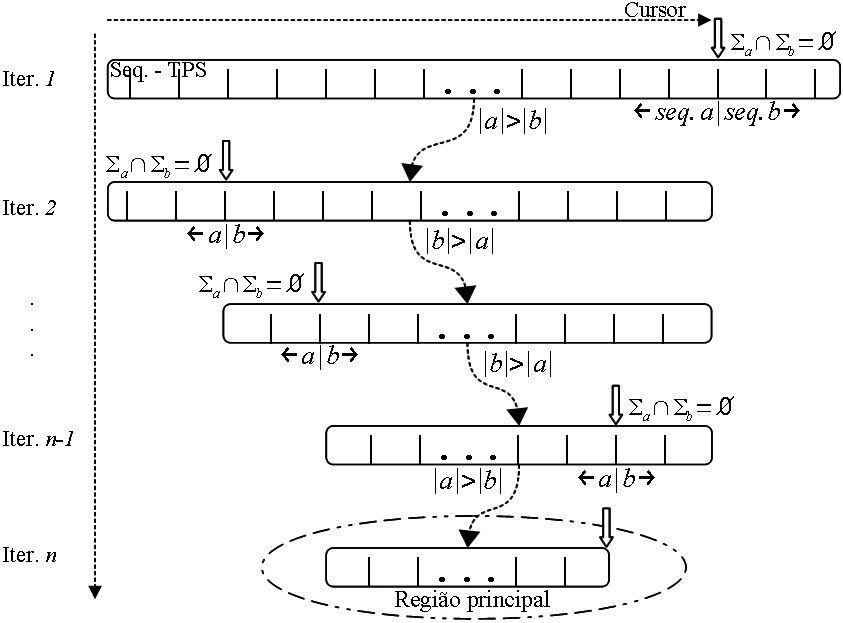
\includegraphics[scale=0.36]{img/alg-pb-pt.jpg}
\end{figure}
}

\frame{\frametitle{Algoritmo}
\begin{figure}[H]
  \caption{Detecção da região principal em uma página web real.}
  \label{fig:alg}
  \centering
    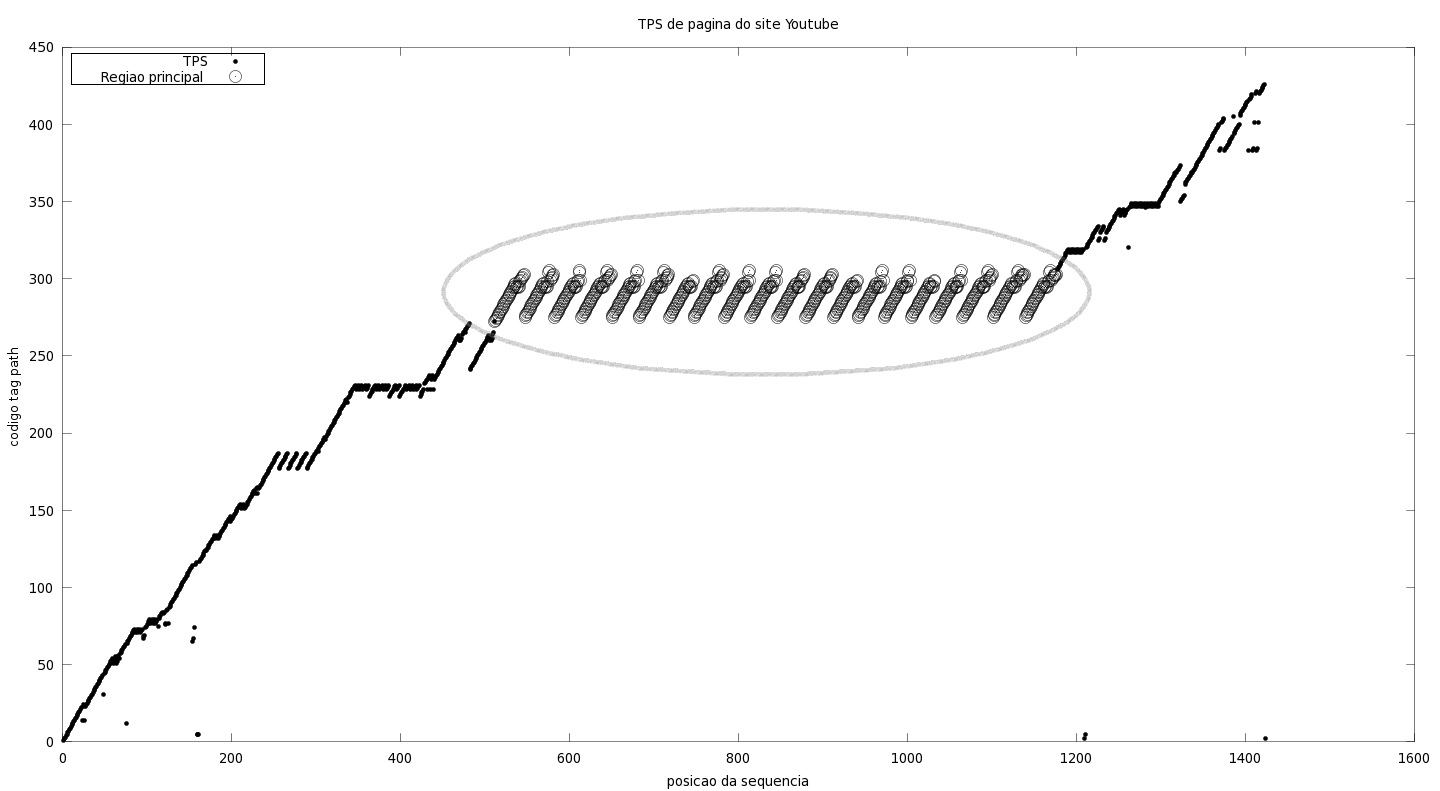
\includegraphics[scale=0.24]{img/tps-pt.jpg}
\end{figure}
}

\frame{\frametitle{Algoritmo}
\begin{figure}[H]
  \caption{Detecção da região principal em uma página web real.}
  \label{fig:ex2}
  \centering
    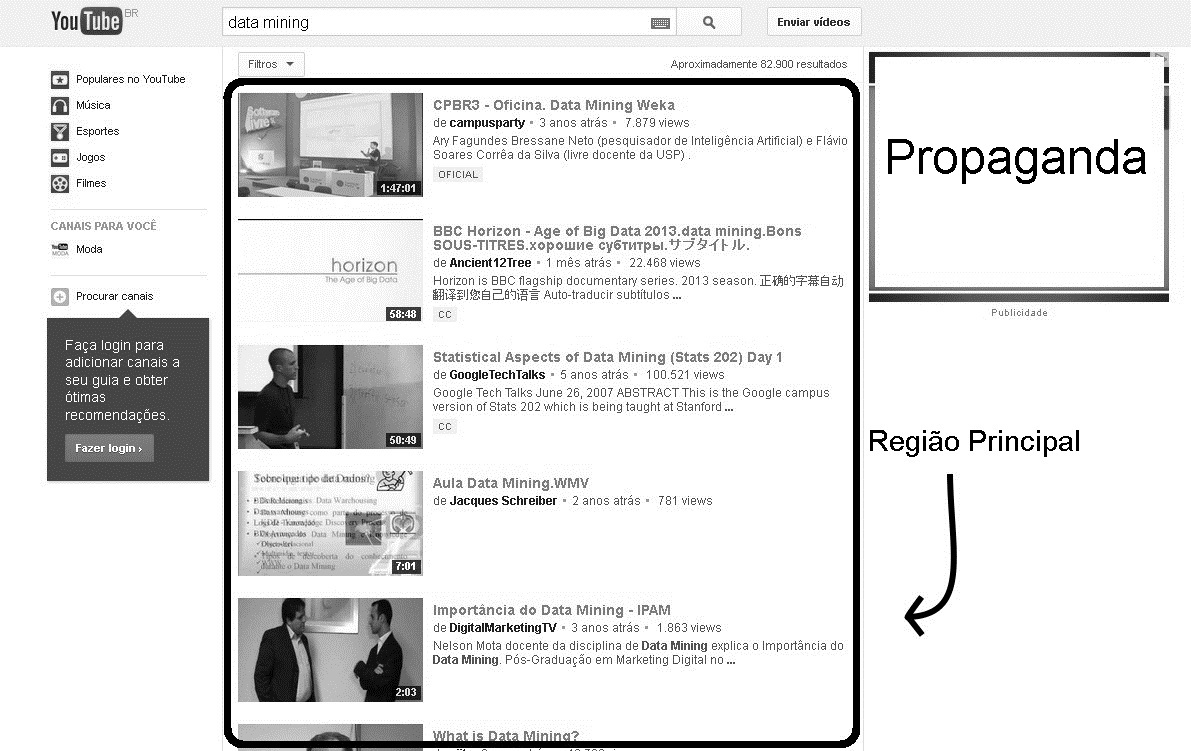
\includegraphics[scale=0.29]{img/example2-gs-pt.jpg}
\end{figure}
}

\begin{frame}[fragile]
\frametitle{Algoritmo - tolerância a ruído}
\fontsize{8}{7.2}\selectfont
\begin{itemize}
\item{HTML code} 
\lstset{numbers=left, language=HTML, frame=single, tabsize=2, caption=Código
HTML, label=lst:html}
\begin{lstlisting}
<body>
	<br> <!-- cabecalho -->
	<div> <!-- menu -->
		<span class='region1'>...</span>
		...
		<span class='region1'>...</span>
	</div> 
	<div> <!-- regiao principal -->
		<span class='region2'>...</span>
		...
		<span class='region2'>...</span>
	</div>
	<div> <!-- publicidade -->
		<span class='region3'>...</span>
		...
		<span class='region3'>...</span>
	</div>
	<br> <!-- rodape -->
</body>
\end{lstlisting}
\item{TPS}
\begin{verbatim}
TPS = (1,2,3,4,...,4,3,5,...,5,3,6,...,6,2)
\end{verbatim}
\item{TPS filtrada}
\begin{verbatim}
TPS = ( , , ,4,...,4, ,5,...,5, ,6,...,6, )
\end{verbatim}
\end{itemize}
\end{frame}

\section{Método} 
%\frame{\tableofcontents[currentsection]}
\frame{\frametitle{Método}
\begin{enumerate}
	\item Escolha de uma técnica de extração estruturada: MDR (LIU; GROSSMAN;
	ZHAI, 2003);
	\item Definição de um conjunto de páginas para teste;
	\item Aplicação da técnica de extração no conjunto de teste, documentando os
	resultados obtidos como $target$ (registro de interesse) ou $noise$
	(ruído);
	\item Nova aplicação da técnica de extração no mesmo conjunto de teste, mas
	desta vez filtrando-o antes, utilizando a técnica proposta neste trabalho,
	documentando os resultados da mesma maneira;
	\item Comparação de ambos os resultados e medição do aumento/redução da
	precisão (remoção de ruído).
\end{enumerate} 
}

\frame{\frametitle{Método}
\begin{figure}[H]
  \caption{Método de avaliação e comparação dos resultados.}
  \label{fig:alg}
  \centering
    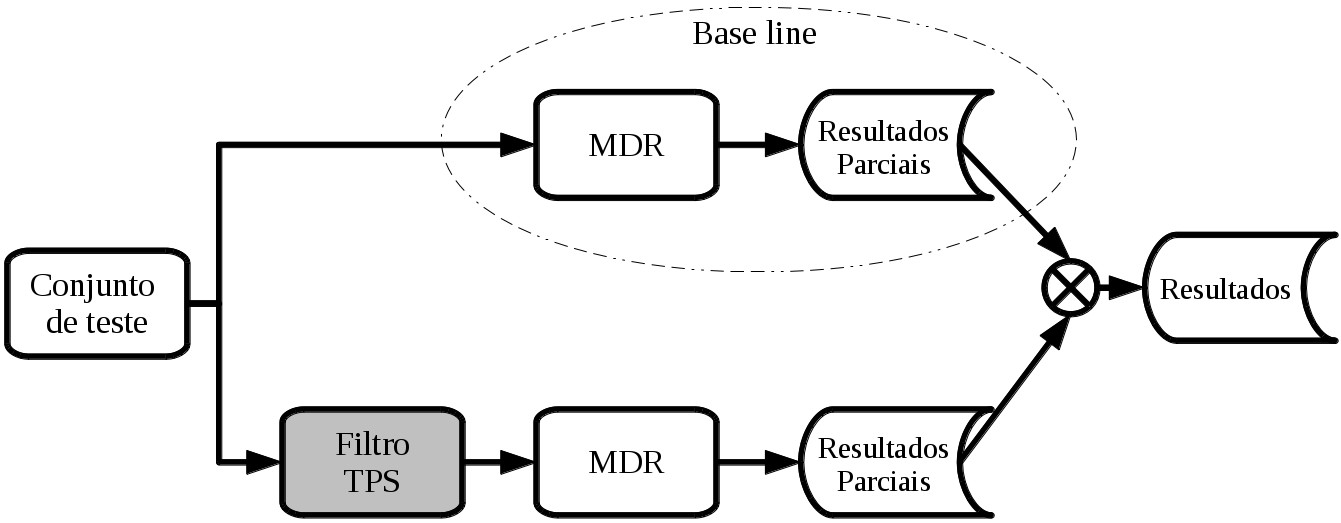
\includegraphics[scale=0.20]{img/metodo.jpg}
\end{figure}
}

\section{Resultados} 
%\frame{\tableofcontents[currentsection]}
\frame{\frametitle{Resultados} 
%\begin{figure}[H]
%  \label{fig:res}
%  \centering
%    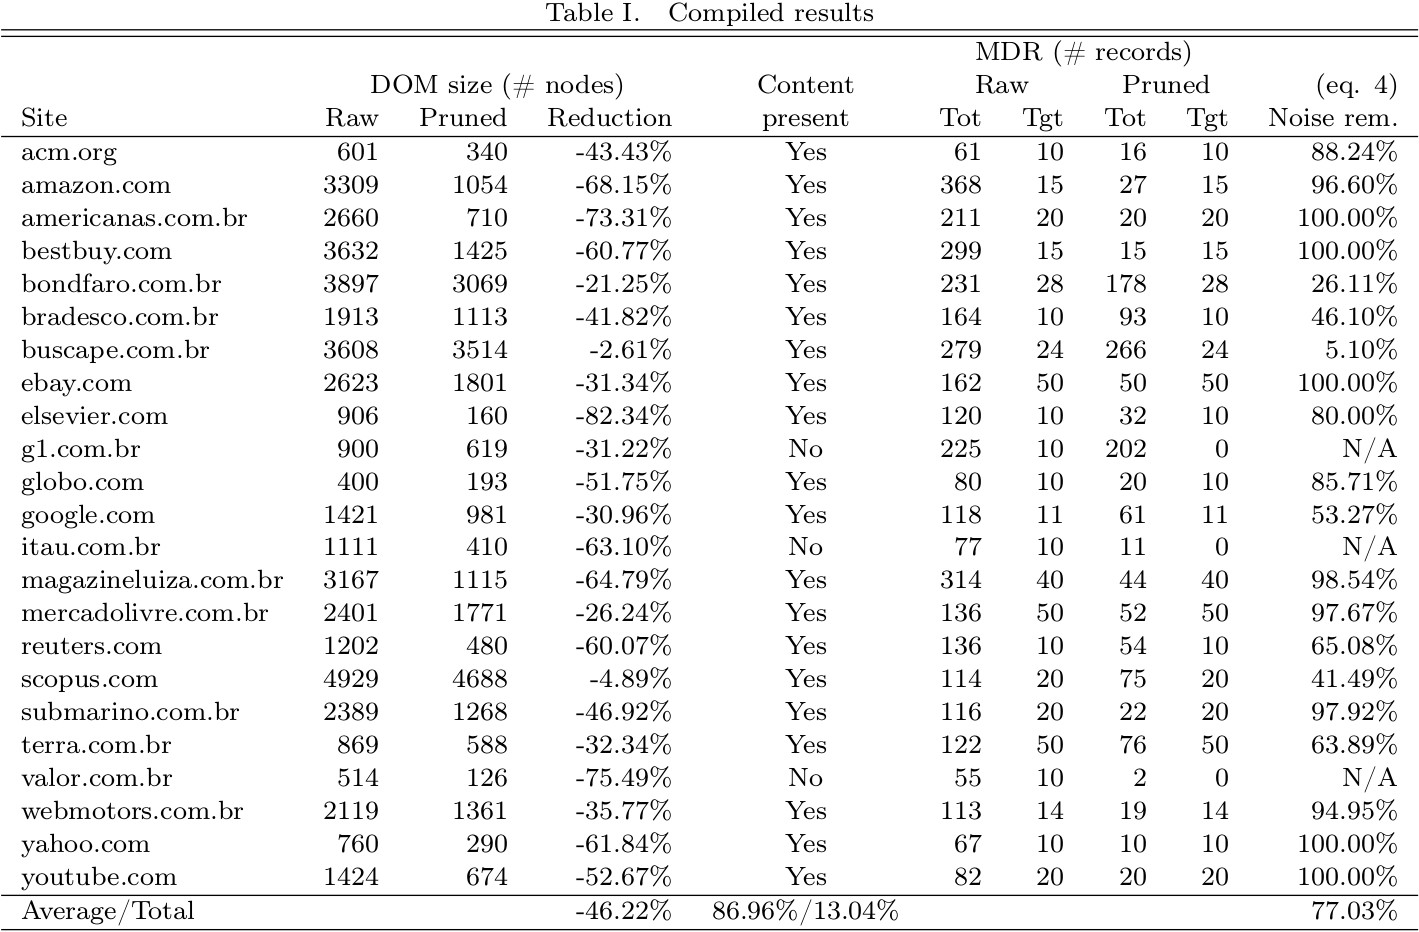
\includegraphics[scale=0.18]{result.jpg}
%\end{figure}


\begin{tiny}
\begin{table}[H]
%\caption{Resultados}
\label{table:results}
\centering
\fontsize{4.8}{0}\selectfont
\begin{tabular}{p{1mm}| p{12mm}| p{3mm} p{6mm} p{9mm}| p{6mm}| p{2mm} p{2mm} |
p{2mm} p{2mm} |r} 
\hline\hline & \multicolumn{5}{c}{} & \multicolumn{4}{c}{MDR (\# registros)} & \\
& & \multicolumn{3}{c}{Tam. DOM (\# nós)} & Cont. & \multicolumn{2}{c}{Orig.}
& \multicolumn{2}{c}{Podado} & Ruído\\
\# & $Site$ & Orig. & Podado & Red. & princ. & Tot & Tgt & Tot & Tgt & rem. \\
\hline
1 & ACM & 601 & 340 & -43,43\% & Sim & 61 & 10 & 16 & 10 & 88,24\% \\
2 & Amazon & 3499 & 1069 & -69,45\% & Sim & 344 & 16 & 41 & 16 & 92,38\% \\
3 & Apple & 1422 & 962 & -32,35\% & Sim & 63 & 15 & 23 & 15 & 83,33\% \\
4 & Avon & 911 & 575 & -36,88\% & Sim & 69 & 20 & 29 & 20 & 81,63\% \\
5 & Barnes \& Noble & 1242 & 778 & -37,36\% & Sim & 147 & 30 & 54 & 30 & 79,49\% \\
6 & Bestbuy & 3632 & 1425 & -60,77\% & Sim & 299 & 15 & 15 & 15 & 100,00\% \\
7 & Blockbuster & 2176 & 1381 & -36,53\% & Sim & 84 & 25 & 32 & 25 & 88,14\% \\
8 & Bondfaro & 3897 & 1820 & -53,30\% & Sim & 160 & 28 & 30 & 28 & 98,48\% \\
9 & Bradesco & 1913 & 1113 & -41,82\% & Sim & 164 & 10 & 93 & 10 & 46,10\% \\
10 & Build & 2712 & 746 & -72,49\% & Não & 117 & 12 & 69 & 0 & N/A \\
11 & Buscapé & 3608 & 1607 & -55,46\% & Sim & 223 & 24 & 24 & 24 & 100,00\% \\
12 & Costco & 4504 & 326 & -92,76\% & Não & 246 & 96 & 8 & 8 & N/A \\
13 & Dell & 1737 & 881 & -49,28\% & Sim & 177 & 12 & 64 & 12 & 68,48\% \\
14 & Disney & 2778 & 2006 & -27,79\% & Sim & 193 & 96 & 116 & 96 & 79,38\% \\
15 & Drugstore & 1774 & 850 & -52,09\% & Sim & 156 & 18 & 52 & 18 & 75,36\% \\
16 & eBay & 2623 & 1801 & -31,34\% & Sim & 162 & 50 & 50 & 50 & 100,00\% \\
17 & Elsevier & 906 & 160 & -82,34\% & Sim & 120 & 10 & 32 & 10 & 80,00\% \\
18 & Footlocker & 2440 & 1106 & -54,67\% & Sim & 238 & 60 & 60 & 60 & 100,00\% \\
19 & Gamestop & 1947 & 935 & -51,98\% & Não & 86 & 12 & 6 & 0 & N/A \\
20 & Gap & 2249 & 1365 & -39,31\% & Sim & 235 & 124 & 126 & 124 & 98,20\% \\
21 & Globo & 400 & 193 & -51,75\% & Sim & 80 & 10 & 20 & 10 & 85,71\% \\
22 & Globo G1 & 900 & 619 & -31,22\% & Não & 225 & 10 & 202 & 0 & N/A \\
23 & Google & 1421 & 474 & -66,64\% & Sim & 118 & 11 & 21 & 11 & 90,65\% \\
24 & Home Depot & 5199 & 1304 & -74,92\% & Sim & 325 & 24 & 24 & 24 & 100,00\% \\
25 & HP & 1783 & 1258 & -29,44\% & Sim & 71 & 15 & 15 & 15 & 100,00\% \\
26 & Itaú & 1111 & 410 & -63,10\% & Não & 77 & 10 & 11 & 0 & N/A \\
27 & Lojas Americanas & 2660 & 710 & -73,31\% & Sim & 211 & 20 & 20 & 20 & 100,00\% \\
28 & Macy's & 5676 & 2158 & -61,98\% & Não & 164 & 40 & 43 & 0 & N/A \\
29 & Magazine Luiza & 3167 & 1115 & -64,79\% & Sim & 314 & 40 & 44 & 40 & 98,54\% \\
30 & Mercadolivre & 2401 & 1771 & -26,24\% & Sim & 136 & 50 & 52 & 50 & 97,67\% \\
31 & Microsoft & 871 & 272 & -68,77\% & Sim & 57 & 16 & 16 & 16 & 100,00\% \\
32 & Newegg & 8481 & 3419 & -59,69\% & Não & 965 & 20 & 307 & 0 & N/A \\
33 & Nike & 4082 & 1829 & -55,19\% & Sim & 329 & 23 & 23 & 23 & 100,00\% \\
34 & Office Depot & 3363 & 1111 & -66,96\% & Sim & 108 & 24 & 38 & 24 & 83,33\% \\
35 & PC Mall & 4285 & 2548 & -40,54\% & Sim & 216 & 25 & 53 & 25 & 85,34\% \\
36 & Rakuten & 3386 & 2768 & -18,25\% & Sim & 112 & 35 & 61 & 35 & 66,23\% \\
37 & Ralph Lauren & 995 & 564 & -43,32\% & Sim & 46 & 12 & 12 & 12 & 100,00\% \\
38 & Reuters & 1202 & 198 & -83,53\% & Sim & 136 & 10 & 10 & 10 & 100,00\% \\
39 & Scopus & 4929 & 4688 & -4,89\% & Sim & 114 & 20 & 75 & 20 & 41,49\% \\
40 & Sears & 5726 & 3890 & -32,06\% & Sim & 397 & 50 & 75 & 50 & 92,80\% \\
41 & Sephora & 3022 & 1440 & -52,35\% & Sim & 365 & 60 & 60 & 60 & 100,00\% \\
42 & Sony & 2200 & 1316 & -40,18\% & Sim & 98 & 15 & 18 & 15 & 96,39\% \\
43 & Staples & 2959 & 1611 & -45,56\% & Sim & 178 & 24 & 24 & 24 & 100,00\% \\
44 & Submarino & 2389 & 1268 & -46,92\% & Sim & 116 & 20 & 22 & 20 & 97,92\% \\
45 & Terra & 869 & 588 & -32,34\% & Sim & 122 & 50 & 76 & 50 & 63,89\% \\
46 & Tiffany & 3899 & 2753 & -29,39\% & Não & 183 & 12 & 67 & 0 & N/A \\
47 & Valor Econômico & 514 & 126 & -75,49\% & Não & 55 & 10 & 2 & 0 & N/A \\
48 & Wal-Mart & 1576 & 808 & -48,73\% & Sim & 110 & 20 & 40 & 20 & 77,78\% \\
49 & Webmotors & 2119 & 1361 & -35,77\% & Sim & 113 & 14 & 19 & 14 & 94,95\% \\
50 & Yahoo! & 760 & 290 & -61,84\% & Sim & 67 & 10 & 10 & 10 & 100,00\% \\
51 & YouTube & 1424 & 674 & -52,67\% & Sim & 82 & 20 & 20 & 20 & 100,00\% \\
\hline
& Média/Total &  &  & -50,18\% & 82,35\%&  &  &  &  & 88,86\% \\
&             &  &  &          & 17,65\%&  &  &  &  &  \\
\hline

\end{tabular}
\end{table}
\end{tiny}

}

\frame{\frametitle{Resultados} 

\begin{small}
\begin{table}[H]
\centering
%\caption{\textit{Precision, recall e F-measure}.}
\label{table:prec}
\begin{tabular}{l l l l}
\hline\hline
& MDR ($a$) & MDR+filtro ($b$) & Variação ($b-a$)\\
\hline
Precisão & 18,93\%  & 75,08\% & 56,15\% \\
$Recall$   & 100,00\% & 82,35\% & -17,65\% \\
F-$measure$ & 31,83\% & 78,55\% & 46,72\% \\
\hline
\end{tabular}
\end{table}
\end{small}
}

\section{Limitações} 
%\frame{\tableofcontents[currentsection]}
\frame{\frametitle{Limitações}
\begin{itemize}
	\item Páginas muito homogêneas;
	\item Páginas muito heterogêneas;
	\item Páginas onde o conteúdo principal é menor que o ruído (17,65\%).
\end{itemize}
}

\section{Trabalhos futuros}
%\frame{\tableofcontents[currentsection]}
\frame{\frametitle{Conclusão e Trabalhos futuros}
\begin{itemize}
  \item Incremento considerável na qualidade da extração; 
  \item Combinar com outras abordagens (semânticas);
  \item Generalizar mais a hipótese sobre páginas com conteúdo estruturado. 
\end{itemize}
}

\end{document}
